% -*- coding: UTF-8 -*-
% vim: autoindent expandtab tabstop=4 sw=4 sts=4 filetype=tex
% chktex-file 27 - disable warning about missing include files

\section{Modelle zur Schattierung (shading models)}
\label{sec:shading}

% * Lighting model at each vertex, e.g. Lambert
% * Shading: Compute the color of interior points between vertices
% * Example image of mesh (vertices)

Sofern nicht anders vermerkt, basieren die nachfolgenden Abschnitte
auf~\cite{foley_computer_1996}[S. 734–739] sowie~\cite{hughes_computer_2013}.

Bei der Anwendung von Modellen zur Schattierung (shading models) geht es
grundsätzlich darum die emitierte Lichtintensität bzw.\ die Farbe einer
Oberfläche an einem bestimmten Punkt zu berechnen. Es wäre naheliegend
dies für jeden sichtbaren Punkt der Oberfläche zu berechnen, dies ist
jedoch häufig viel zu aufwändig. Viele Modelle zur Schattierung
berechnen daher die Licht- bzw. Farbintensität nur an gewissen
Schlüsselpunkten und wenden dann vereinfachte Modelle zur Berechnung an
um so Rechenzeit zu sparen.

Als Beispiel zur Anwendung der Schattierungsmodelle wird nachfolgend
angenommen, dass mittels einem Beleuchtungsmodell an jedem Eckpunkt einer
Oberfläche (Polygon) die Farbe berechnet wird. Als Beispiel dienen hier die
Eckpunkte $\bm{V}_{1}$, $\bm{V}_{2}$, $\bm{V}_{3}$ und $\bm{V}_{4}$.

\begin{figure}[H]
    \centering
    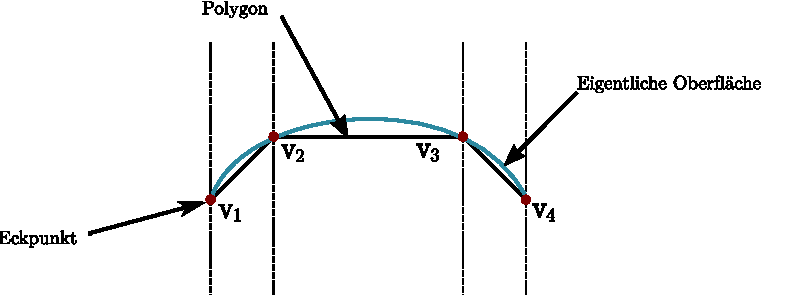
\includegraphics{img/shading_mesh.pdf}
    \caption{Illustration der Ausgangslage\protect\footnotemark}\label{
        fig:shading_mesh_illustration}
\end{figure}
\footnotetext{Eigene Darstellung mittels Inkscape, angelehnt
    an~\cite{hughes_computer_2013}}

Um einen Farbintensitätswert für einen Eckpunkt $\bm{V}_{1}$ zu berechnen, wird der
Normalenvektor des Eckpunktes (vertex normal) benötigt. Es handelt sich dabei
um den Normalenvektor der Oberfläche an der Position des Eckpunktes $\bm{V}_{1}$.

Im Laufe der Zeit hat sich die Schattierung so weit entwickelt, dass
diese praktisch ausschliesslich auf der Grafikkarte (GPU) statt findet.
Man spricht hier vom Begriff ``Shader''. Es handelt sich dabei
mittlerweile um eigene (Grafik-) Applikationen, deren Zweck weit über
die reine Berechnung von Schattierungen hinausgeht.  Man unterscheidet
dabei zwischen Shadern für geometrische Berechnungen (\textit{geometry
    shaders} oder \textit{vertex shaders}) sowie Shader für Berechnungen
bezüglich Pixeln  oder (Bild-) Fragmenten (\textit{pixel shaders} oder
\textit{fragment shaders}).~\cite{hughes_computer_2013}[Kapitel 33]\\
Der interessierte Leser sei für weitere Details
auf~\cite{hughes_computer_2013}[Kapitel
33],~\cite{opengl_foundation_rendering_2015},
sowie~\cite{fernando_cg_2003} verwiesen.

\subsection{Flat-Shading --- per vertex lighting}
\label{subsec:flat_shading}

% * Calculate normal for each vertice by averaging line-segment normals, e.g.
%   (normal(V1V2) + normal(V3V4)) / 2 to determine per vertex color
%   * Image of calculated normals: line-segment (given through mesh) and vertex
% * One color per face determined by vertex' color

Bei Flat-Shading wird pro Oberfläche (Polygon) ein Eckpunkt $\bm{V}_{1}$ dieser als
farb- bzw.\ intensitätgebender Schlüsselpunkt bestimmt. Danach wird die Farbe
des Punktes als Farbe für die Oberfläche genommen.

Diese Annahme ist unter den folgenden Voraussetzungen gültig:
\begin{enumerate}
    \item{Die zugrundeliegende Lichtquelle befindet sich unendlich weit
            entfernt, so dass der Winkel zwischen dem
            Normalenvektor der Oberfläche und der Lichtquelle
            $\bm{n}\cdot{}\bm{l}$ für die gesamte Oberfläche konstant ist.}
    \item{Der Betrachter sich unendlich weit entfernt von der Oberfläche
            befindet, so dass der Winkel zwischen dem Normalenvektor der
            Oberfläche und dem Betrachter $\bm{n}\cdot{}\bm{v}$ für die
            gesamte Oberfläche konstant ist.}
    \item{Das Polygon ist eine effektive Repräsentation der Oberfläche
            und nicht nur eine Näherung einer runden Oberfläche.}
\end{enumerate}

\begin{figure}[H]
    \centering
    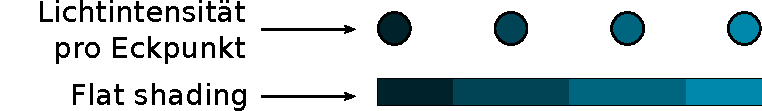
\includegraphics{img/flat_shading.pdf}
    \caption{Illustration des Flat-Shadings\protect\footnotemark}\label{
        fig:flat_shading_illustration}
\end{figure}
\footnotetext{Eigene Darstellung mittels Inkscape, angelehnt
    an~\cite{hughes_computer_2013}}

Ist eine der ersten beiden Annahmen falsch, so muss für den Vektor der
Lichtquelle $\bm{l}$ bzw.\ den Vektor des Betrachters $\bm{v}$ ein
konstanter Wert berechnet werden.~\citeauthor{foley_computer_1996} gibt
hier als Beispiele das Zentrum des Polygones oder den ersten Eckpunkt
des Polygones an.

\subsection{Gouraud-Shading --- face interpolated lighting}
\label{subsec:gouraud_shading}

Bei Gouraud-Shading handelt es sich um ein Shading-Verfahren, welches die
Farbintensitätswerte der Eckpunkte von Oberflächen eines Meshes interpoliert.

\begin{figure}[H]
    \centering
    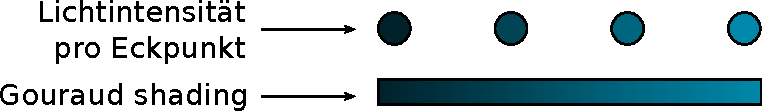
\includegraphics{img/gouraud_shading.pdf}
    \caption{Illustration des Gouraud-Shadings\protect\footnotemark.}\label{
        fig:gouraud_shading_illustration}
\end{figure}
\footnotetext{Eigene Darstellung mittels Inkscape, angelehnt
    an~\cite{hughes_computer_2013}}

Um den Farbintensitätswert eines Eckpunktes von Oberflächen  zu berechnen,
schlägt Gouraud die Berechnung des Durchschnittswertes der Oberflächennormalen
zweier adjazenter Liniensegmente (im 2D-Raum) bzw.\  aller adjazenter Dreiecke
(im 3D-Raum) vor.

\begin{figure}[H]
    \centering
    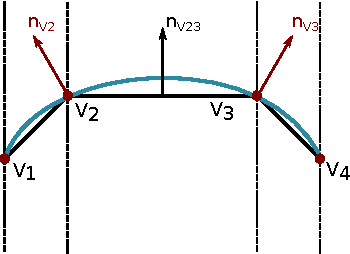
\includegraphics{img/shading_mesh_normals.pdf}
    \caption{Illustration der berechneten Normalenvektoren $\bm{n}_{v_{2}}$ und
    $\bm{n}_{v_{3}}$ an den Eckpunkten $v_{2}$ und $v_{3}$ sowie des
    Normalenvektors $\bm{n}_{v_{23}}$ der Kante $\bm{v_{2}v_{3}}$
    \protect\footnotemark.}\label{fig:gouraud_shading_normals_illustration}
\end{figure}
\footnotetext{Eigene Darstellung mittels Inkscape, angelehnt
    an~\cite{hughes_computer_2013}}

Die Berechnung des Normalenvektors eines Eckpunktes via Durchschnittswert ist
üblicherweise eine genügend gute Näherung der Oberflächennormale der
eigentlichen Oberfläche. Die Präzision hängt dabei aber klar von der
Granularität des Modelles (Mesh) ab.

\subsection{Phong-Shading --- normal interpolated lighting}
\label{subsec:phong_shading}

Phong-Shading ist eine Verbesserung des Gouraud-Verfahrens und bietet eine
bessere Annäherung an die Schattierung bzw. Darstellung von glatten
Oberflächen. Das Verfahren eignet sich vor allem dann besser, wenn ein
Beleuchtungsmodell verwendet wird, welches kleine spekuläre Refelektionen
bietet, wie z.B. das Phong-Beleuchtungsmodell.

Bei Phong-Shading wird ein Normalenvektor linear an einer Oberfläche (eines
Polygons) interpoliert, ausgehend von den Normalenvektoren der Kanten der
Oberfläche (im obigen Beispiel wäre dies $\bm{n}_{v_{2}v_{3}}$). Die
Oberflächennormale wird an jedem Pixel interpoliert und normalisiert und kommt
dann für die Berechnung des Farbintnsitätswertes anhand eines
Beleuchtungsmodelles, wie zum Beispiel das Phong-Beleuchtungsmodell, zum
Einsatz. Daher ist Phong-Shading viel rechenaufwändiger als Gouraud-Shading, da
das Beleuchtungsmodell für jeden Pixel anstatt für jede Kante berechnet werden
muss.

\begin{figure}[H]
    \centering
    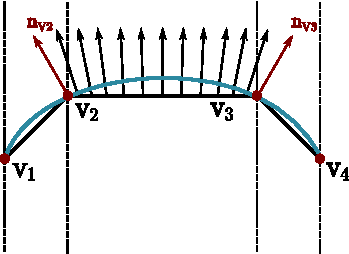
\includegraphics{img/phong_shading_mesh_normals.pdf}
    \caption{Stark vereinfachte Illustration der interpolierten
        Normalenvektoren anhand der Kante $\bm{v_{2}v_{3}}$
    \protect\footnotemark.}\label{fig:phong_shading_normals_illustration}
\end{figure}
\footnotetext{Eigene Darstellung mittels Inkscape, angelehnt
    an~\cite{hughes_computer_2013}}


\begin{table}[H]
    \centering
    \caption{Vergleich der genannten Shading-Verfahren anhand einer
    Beispielszene\protect\footnotemark.}\label{table:shading_comparision}
    \begin{tabular}{p{0.2\textwidth}p{0.2\textwidth}p{0.2\textwidth}p{0.2\textwidth}}
        \toprule
            \textbf{Flat-Shading} &
            \textbf{Gouraud-Shading} &
            \textbf{Gouraud-Shading mit Phong-Beleuchtungsmodell} &
            \textbf{Phong-Shading mit Phong-Beleuchtungsmodell} \\
            \cmidrule(r){1-1}\cmidrule(lr){2-2}\cmidrule(lr){3-3}\cmidrule(l){4-4}
            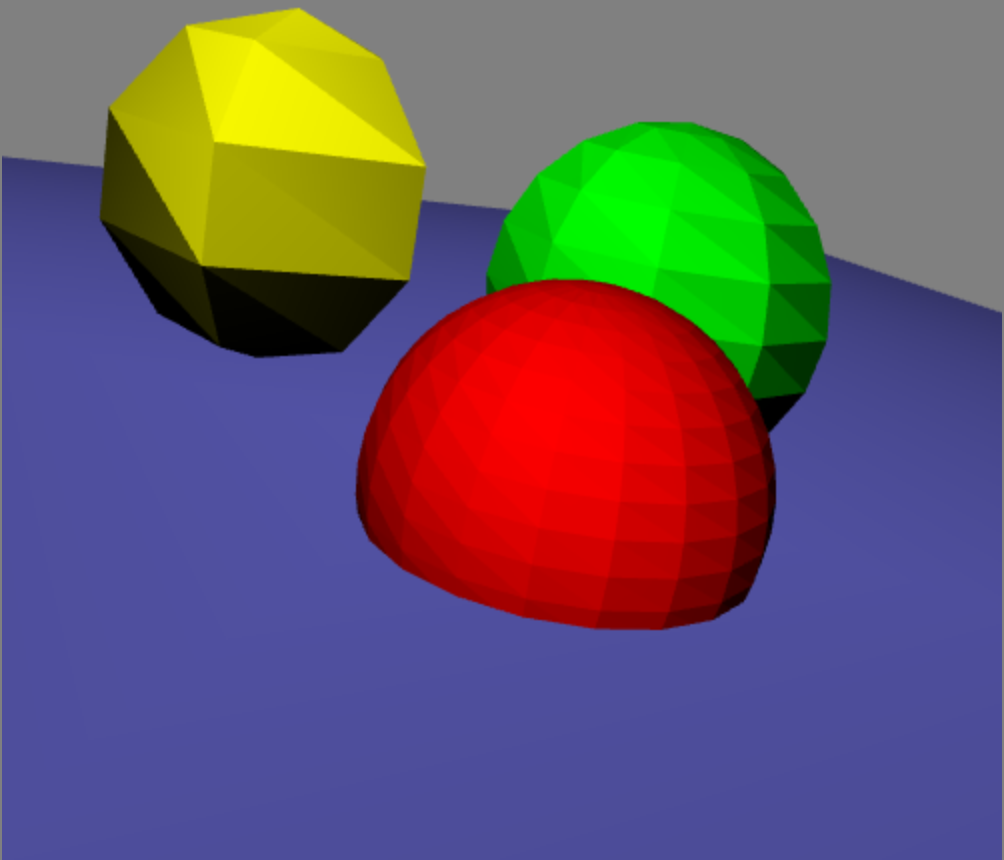
\includegraphics[width=0.2\textwidth]{img/flat_shading_example.png} \newline &
            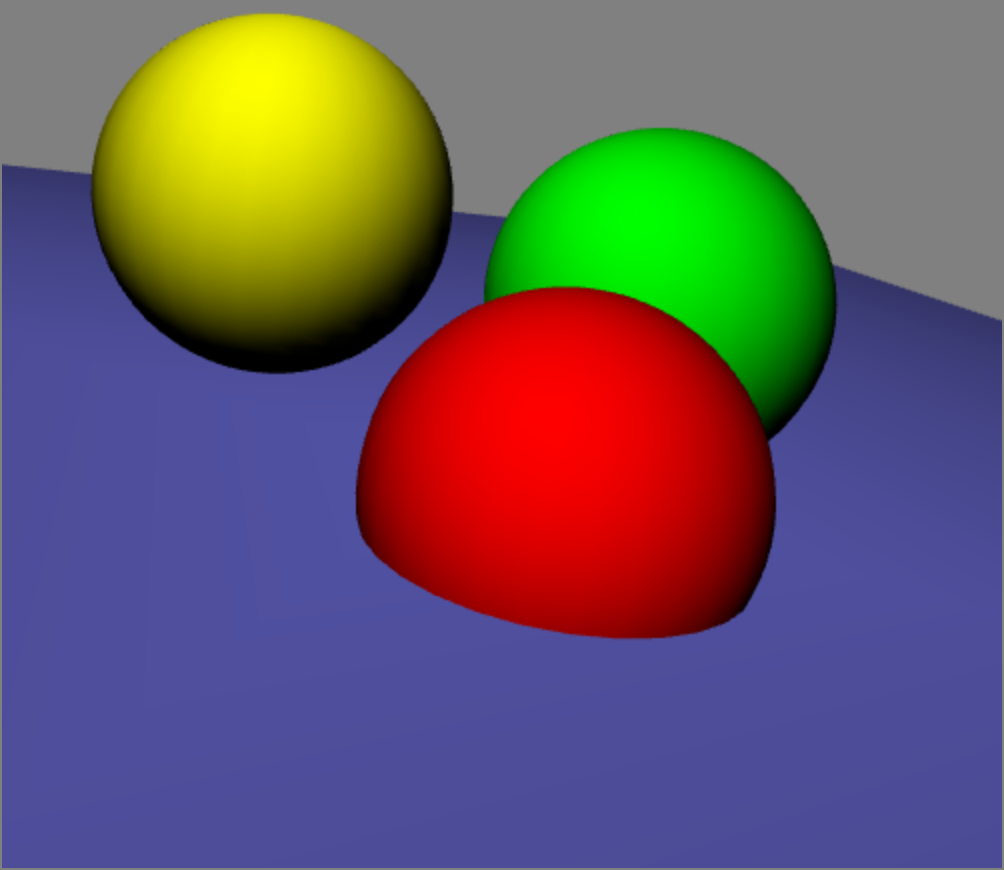
\includegraphics[width=0.2\textwidth]{img/gouraud_shading_example.png} \newline &
            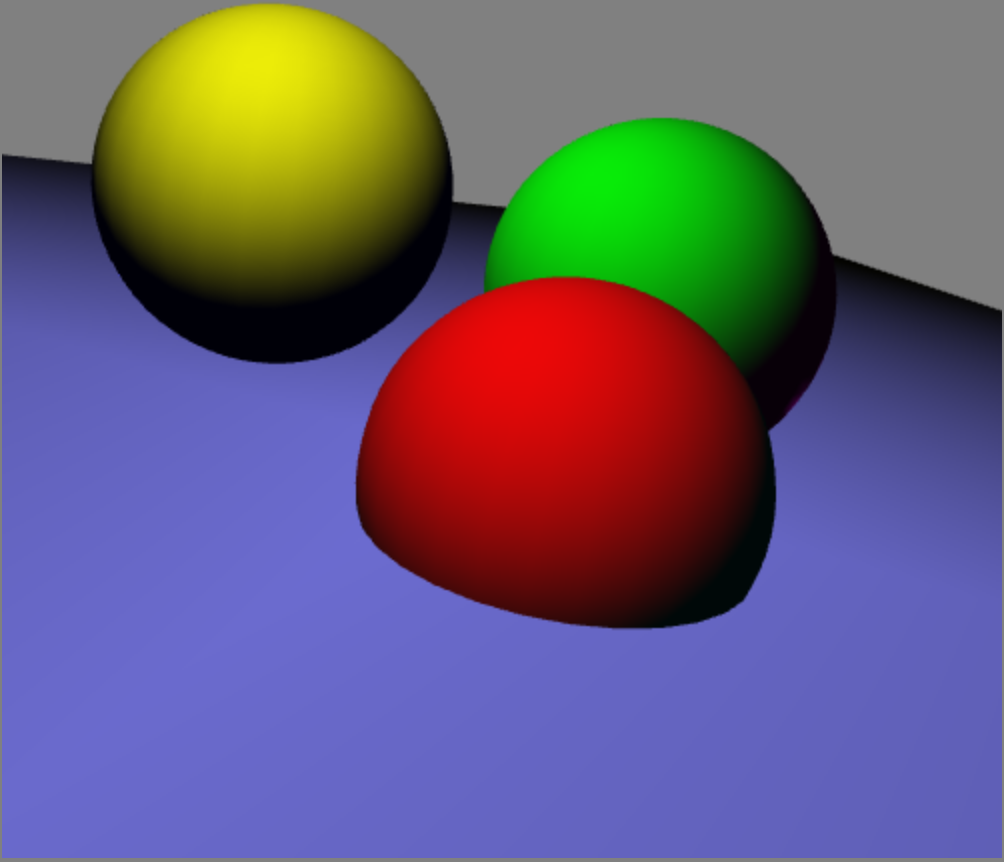
\includegraphics[width=0.2\textwidth]{img/phong_gouraud_shading_example.png} \newline &
            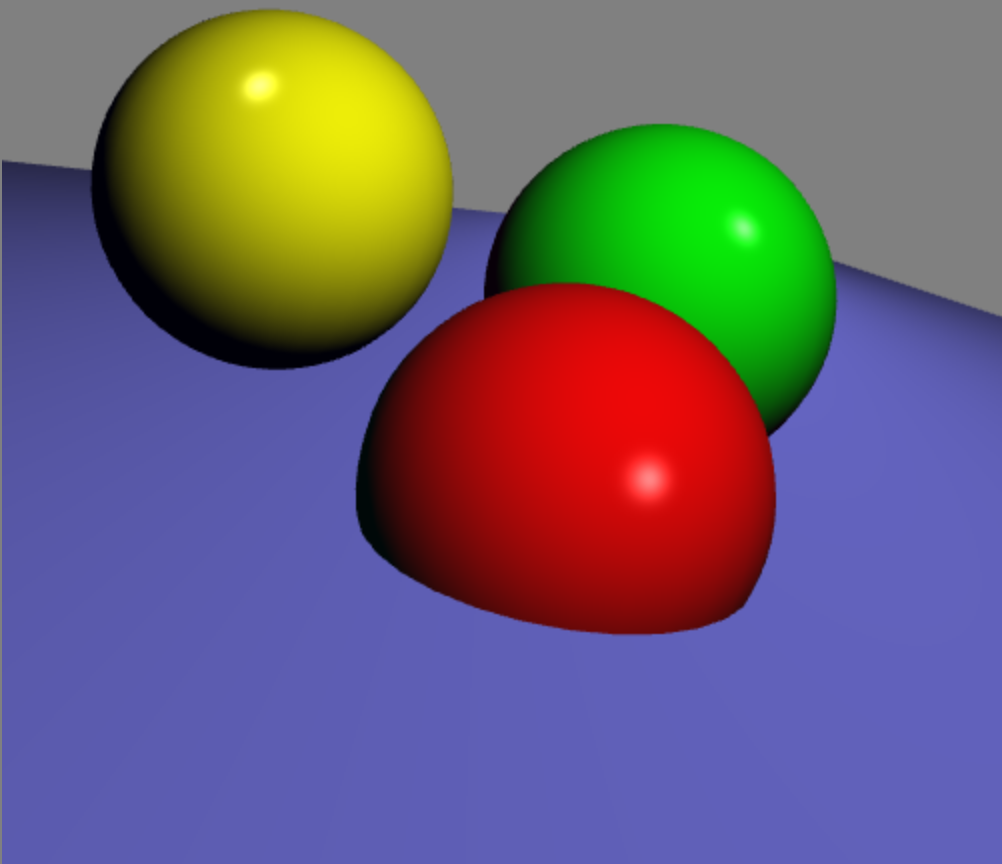
\includegraphics[width=0.2\textwidth]{img/phong_phong_shading_example.png} \newline \\
        \bottomrule
    \end{tabular}
\end{table}
\footnotetext{\cite{danchilla_beginning_webgl}}
